\section{绝对收敛与条件收敛}
\subsection{绝对收敛与条件收敛的概念}
\begin{definition}
%@see: 《高等数学(第六版 下册)》 P263
%@see: 《数学分析(第二版 下册)》(陈纪修) P35 定义9.4.2
设级数\(\sum_{n=1}^\infty u_n\)的各项为任意实数.
\begin{itemize}
	\item 如果级数\(\sum_{n=1}^\infty \abs{u_n}\)收敛,
	则称“级数\(\sum_{n=1}^\infty u_n\)~\DefineConcept{绝对收敛}”.
	\item 如果级数\(\sum_{n=1}^\infty u_n\)收敛,
	而级数\(\sum_{n=1}^\infty \abs{u_n}\)发散,
	则称“级数\(\sum_{n=1}^\infty u_n\)~\DefineConcept{条件收敛}”.
\end{itemize}
\end{definition}

\begin{example}
%@see: 《数学分析(第二版 下册)》(陈纪修) P35
\(\sum_{n=1}^\infty \frac{(-1)^{n+1}}n\)是一个条件收敛级数.
\end{example}

\begin{theorem}\label{theorem:无穷级数.绝对收敛级数必定收敛}
%@see: 《高等数学(第六版 下册)》 P263 定理8
%@see: 《数学分析教程 (第3版 下册)》(史济怀) P188 定理14.5.1
%@see: 《数学分析(第二版 下册)》(陈纪修) P36 定理9.4.4
设\(\{u_n\}\)是实数列,
令\(v_n \defeq \frac12 (u_n + \abs{u_n}),
w_n \defeq \frac12 (\abs{u_n} - u_n)
\ (n=1,2,\dotsc)\).
\begin{itemize}
	\item 如果级数\(\sum_{n=1}^\infty u_n\)绝对收敛,
	则级数\(\sum_{n=1}^\infty u_n\)、\(\sum_{n=1}^\infty v_n\)和\(\sum_{n=1}^\infty w_n\)都收敛.

	\item 如果级数\(\sum_{n=1}^\infty u_n\)条件收敛,
	则级数\(\sum_{n=1}^\infty v_n\)和\(\sum_{n=1}^\infty w_n\)都发散.
\end{itemize}
\begin{proof}
可见级数\(\sum_{n=1}^\infty v_n\)是
级数\(\sum_{n=1}^\infty u_n\)中的全体正项所构成的级数,
而级数\(\sum_{n=1}^\infty w_n\)是
级数\(\sum_{n=1}^\infty u_n\)中全体负项的绝对值所构成的级数.
级数\(\sum_{n=1}^\infty v_n\)和\(\sum_{n=1}^\infty w_n\)都是正项级数.

先设级数\(\sum_{n=1}^\infty u_n\)绝对收敛,
由于\[
	0 \leq v_n \leq \abs{u_n},
	0 \leq w_n \leq \abs{u_n},
	\quad n=1,2,\dotsc,
\]
所以由\hyperref[theorem:无穷级数.正项级数的比较审敛法]{比较审敛法}可知
级数\(\sum_{n=1}^\infty v_n\)和\(\sum_{n=1}^\infty w_n\)都收敛.
又因为\[
	u_n = v_n - w_n,
\]
所以由\hyperref[theorem:无穷级数.收敛级数性质2]{收敛级数的基本性质}可知\[
	\sum_{n=1}^\infty u_n
	= \sum_{n=1}^\infty v_n
	- \sum_{n=1}^\infty w_n,
\]
那么级数\(\sum_{n=1}^\infty u_n\)收敛.

再设级数\(\sum_{n=1}^\infty u_n\)条件收敛.
用反证法,假设级数\(\sum_{n=1}^\infty v_n\)也收敛,
则由\[
	w_n = \frac12 (\abs{u_n} - u_n)
	= \frac12 (u_n + \abs{u_n} - 2 u_n)
	= v_n - u_n,
\]可知\[
	\sum_{n=1}^\infty w_n
	= \sum_{n=1}^\infty v_n
	- \sum_{n=1}^\infty u_n,
\]
所以级数\(\sum_{n=1}^\infty w_n\)也收敛,
于是级数\[
	\sum_{n=1}^\infty \abs{u_n}
	= \sum_{n=1}^\infty v_n
	+ \sum_{n=1}^\infty w_n
\]也收敛,与假设矛盾!
因此级数\(\sum_{n=1}^\infty v_n\)必定发散.
同理级数\(\sum_{n=1}^\infty w_n\)也必定发散.
\end{proof}
\end{theorem}

建立\cref{theorem:无穷级数.绝对收敛级数必定收敛} 以后,
我们就把一大类级数的收敛性判定问题,
转化成为正项级数的收敛性判定问题.

一般说来,
如果级数\(\sum_{n=1}^\infty \abs{u_n}\)发散,
我们不能断定级数\(\sum_{n=1}^\infty u_n\)也发散.
正如我们在\cref{example:无穷级数.交错级数1} 看到的那样,
虽然\(\sum_{n=1}^\infty \frac{1}{n}\)发散,
但是\(\sum_{n=1}^\infty \frac{(-1)^{n+1}}{n}\)收敛.
但是,如果我们用比值审敛法或根值审敛法,
根据\(\lim_{n\to\infty} \abs{\frac{u_{n+1}}{u_n}} > 1\)
或\(\lim_{n\to\infty} \sqrt[n]{\abs{u_n}} > 1\)
判定级数\(\sum_{n=1}^\infty \abs{u_n}\)发散,
那么我们可以断定级数\(\sum_{n=1}^\infty u_n\)必然发散.

\begin{theorem}\label{theorem:无穷级数.绝对发散的特殊情况}
%@see: 《高等数学(第六版 下册)》 P264
当级数\(\sum_{n=1}^\infty u_n\)满足\[
	\lim_{n\to\infty} \abs{\frac{u_{n+1}}{u_n}} = \rho > 1
	\quad\text{或}\quad
	\lim_{n\to\infty} \sqrt[n]{\abs{u_n}} = \rho > 1
\]时,
这个级数必定发散.
\begin{proof}
这是因为从\(\rho > 1\)可推知\(\abs{u_n} \not\to 0\ (n\to\infty)\),
从而\(u_n \not\to 0\ (n\to\infty)\),
因此级数\(\sum_{n=1}^\infty u_n\)是发散的.
\end{proof}
\end{theorem}

\begin{example}
%@see: 《高等数学(第六版 下册)》 P265 例9
判断级数\(\sum_{n=1}^\infty \frac{\sin n\alpha}{n^2}\)的敛散性.
\begin{solution}
因为\[
	\abs{\frac{\sin n\alpha}{n^2}}
	\leq \frac1{n^2},
\]
而级数\(\sum_{n=1}^\infty \frac1{n^2}\)收敛,
所以级数\(\sum_{n=1}^\infty \abs{\frac{\sin n\alpha}{n^2}}\)收敛,
由\cref{theorem:无穷级数.绝对收敛级数必定收敛} 可知,
级数\(\sum_{n=1}^\infty \frac{\sin n\alpha}{n^2}\)收敛.
\end{solution}
\end{example}

\begin{example}
%@see: 《数学分析(第二版 下册)》(陈纪修) P35 例9.4.4
判断级数\(\sum_{n=1}^\infty \frac{x^n}{n^p}\)的敛散性.
\begin{solution}
对\(\sum_{n=1}^\infty \abs{\frac{x^n}{n^p}}
= \sum_{n=1}^\infty \frac{\abs{x}^n}{n^p}\)
应用\hyperref[theorem:无穷级数.正项级数的根值审敛法]{柯西审敛法},有\[
	\lim_{n\to\infty} \sqrt[n]{\frac{\abs{x}^n}{n^p}}
	= \abs{x}.
\]
由此可知:\begin{itemize}
	\item 当\(\abs{x}<1\)时,对于任意实数\(p\),
	总有级数\(\sum_{n=1}^\infty \frac{x^n}{n^p}\)绝对收敛;

	\item 当\(\abs{x}>1\)时,对于任意实数\(p\),
	总有级数\(\sum_{n=1}^\infty \frac{x^n}{n^p}\)发散;

	\item 当\(x=1\)时,
	若\(p>1\)则级数\(\sum_{n=1}^\infty \frac{x^n}{n^p}\)收敛,
	若\(p\leq1\)则级数\(\sum_{n=1}^\infty \frac{x^n}{n^p}\)发散;

	\item 当\(x=-1\)时,
	若\(p>1\)则级数\(\sum_{n=1}^\infty \frac{x^n}{n^p}\)绝对收敛,
	若\(0<p\leq1\)则级数\(\sum_{n=1}^\infty \frac{x^n}{n^p}\)条件收敛,
	若\(p\leq0\)则级数\(\sum_{n=1}^\infty \frac{x^n}{n^p}\)发散.
\end{itemize}
\end{solution}
\end{example}

\begin{example}
%@see: 《数学分析(第二版 下册)》(陈纪修) P36 例9.4.5
判断级数\(\sum_{n=1}^\infty \frac{\sin nx}{n^p}\ (0<x<\pi)\)的敛散性.
\begin{solution}
当\(p>1\)时,由\(\frac{\abs{\sin nx}}{n^p} \leq \frac1{n^p}\),
可知级数\(\sum_{n=1}^\infty \frac{\sin nx}{n^p}\)绝对收敛.

当\(0<p\leq1\)时,
由\cref{example:无穷级数.单调收敛数列与正弦函数列的乘积的级数收敛} 可知
级数\(\sum_{n=1}^\infty \frac{\sin nx}{n^p}\)收敛,
进而有\[
	\frac{\abs{\sin nx}}{n^p}
	\geq \frac{\sin^2nx}{n^p}
	= \frac1{2n^p} - \frac{\cos2nx}{2n^p},
\]
因为级数\(\sum_{n=1}^\infty \frac1{2n^p}\)发散,
所以级数\(\sum_{n=1}^\infty \frac{\abs{\sin nx}}{n^p}\)发散,
级数\(\sum_{n=1}^\infty \frac{\sin nx}{n^p}\)条件收敛.

当\(p\leq0\)时,由于级数的一般项不趋于\(0\),
级数\(\sum_{n=1}^\infty \frac{\sin nx}{n^p}\)发散.
\end{solution}
\end{example}

\begin{example}
%@see: 《高等数学(第六版 下册)》 P265 例10
判断级数\(\sum_{n=1}^\infty (-1)^n \frac1{2^n} \left(1+\frac1n\right)^{n^2}\)的敛散性.
\begin{solution}
记\(u_n = \frac1{2^n} \left(1+\frac1n\right)^{n^2}\),
有\[
	\sqrt[n]{u_n}
	= \frac12 \left(1+\frac1n\right)^n
	\to \frac12 e \quad(n\to\infty),
\]
而\(e/2>1\),所以\(u_n \not\to 0\ (n\to\infty)\),
那么级数\(\sum_{n=1}^\infty (-1)^n \frac1{2^n} \left(1+\frac1n\right)^{n^2}\)发散.
\end{solution}
\end{example}

\begin{example}
已知\(a_n < b_n\ (n=1,2,\dotsc)\),
若级数\(\sum_{n=1}^\infty a_n\)与\(\sum_{n=1}^\infty b_n\)均收敛,
证明:“\(\sum_{n=1}^\infty a_n\)绝对收敛”是
“\(\sum_{n=1}^\infty b_n\)绝对收敛”的充分必要条件.
\begin{proof}
由题可知级数\(\sum_{n=1}^\infty (b_n - a_n)\)是收敛的正项级数,因而绝对收敛.

当级数\(\sum_{n=1}^\infty a_n\)绝对收敛时,
由\hyperref[theorem:不等式.三角不等式1]{三角不等式}有\[
	\abs{b_n} = \abs{(b_n - a_n) + a_n}
	\leq \abs{b_n - a_n} + \abs{a_n},
\]
那么由\hyperref[theorem:无穷级数.正项级数的比较审敛法]{比较审敛法}可知,
\(\sum_{n=1}^\infty \abs{b_n}\)收敛,
\(\sum_{n=1}^\infty b_n\)绝对收敛.

同理,当级数\(\sum_{n=1}^\infty b_n\)绝对收敛时,
亦有\(\sum_{n=1}^\infty a_n\)绝对收敛.
\end{proof}
\end{example}

\subsection{绝对收敛级数的性质}
绝对收敛级数有很多性质是条件收敛级数所没有的.

%@see: 《数学分析(第二版 上册)》(陈纪修) P37 加法交换律
\cref{theorem:无穷级数.收敛级数性质4} 表明:收敛级数保持结合律.
那么,收敛级数是否也保持交换律呢?
也就是说,将一个收敛级数\(\sum_{n=1}^\infty u_n\)的项任意重新排列,
得到一个新级数\(\sum_{n=1}^\infty v_n\)
(我们把级数\(\sum_{n=1}^\infty v_n\)
称为“级数\(\sum_{n=1}^\infty u_n\)的\DefineConcept{更序级数}”),
这个新级数是否仍然收敛?如果这个新级数收敛,其和是否保持不变,即是否有\[
	\sum_{n=1}^\infty v_n = \sum_{n=1}^\infty u_n
\]成立?
遗憾的是,答案是否定的.

%@see: 《数学分析(第二版 上册)》(陈纪修) P37 例9.4.6
考虑莱布尼茨级数\[
	\sum_{n=1}^\infty \frac{(-1)^{n+1}}n.
\]
这是一个条件收敛级数,可以证明它的和为\(\ln2\).
现在重新排列这个级数的项,依次在每一个正项后面接两个负项,即\[
	\sum_{n=1}^\infty u'_n
	= 1 - \frac12 - \frac14
	+ \frac13 - \frac16 - \frac18
	+ \dotsb
	+ \frac1{2n-1} - \frac1{4n-2} - \frac1{4n}
	+ \dotsb.
\]
设\(\sum_{n=1}^\infty \frac{(-1)^{n+1}}n\)的部分和数列为\(\{S_n\}\),
\(\sum_{n=1}^\infty u'_n\)的部分和数列为\(\{S'_n\}\),
则\begin{align*}
	S'_{3n}
	&= \sum_{k=1}^n \left(
		\frac1{2k-1} - \frac1{4k-2} - \frac1{4k}
	\right) \\
	&= \sum_{k=1}^n \left(
		\frac1{4k-2} - \frac1{4k}
	\right) \\
	&= \frac12 \sum_{k=1}^n \left(
		\frac1{2k-1} - \frac1{2k}
	\right)
	= \frac12 S_{2n},
\end{align*}
于是\[
	\lim_{n\to\infty} S'_{3n}
	= \frac12 \lim_{n\to\infty} S_{2n}
	= \frac12 \ln 2.
\]
%TODO QUESTION: 下面为什么要研究\(S'_{3n-1}\)和\(S'_{3n+1}\),我还没想明白!
%TODO {ce603838-a24d-4616-9395-d7b223e8cb72}说\(S'_{3n}\)是\(n=3k\)(模3得0)情况下的部分和,还要考虑模3得1或2的形式
%TODO 下面两条等式说明当\(n\to\infty\)时,\(S'_{3n-1}\)和\(S'_{3n+1}\)两者与\(S'_{3n}\)相比,只是多了一个无穷小
由于\[
	S'_{3n-1} = S'_{3n} + \frac1{4n},
	\qquad
	S'_{3n+1} = S'_{3n} + \frac1{2n+1},
\]
所以\[
	\lim_{n\to\infty} S'_{3n-1}
	= \lim_{n\to\infty} S'_{3n+1}
	= \lim_{n\to\infty} S'_{3n}
	= \frac12 \ln 2.
\]
最终得到\[
	\sum_{n=1}^\infty u'_n
	= \lim_{n\to\infty} S'_n
	= \frac12 \ln 2.
\]
也就是说,尽管级数\(\sum_{n=1}^\infty \frac{(-1)^{n+1}}n\)收敛,但它不保持交换律.

这个例子告诉我们,要使一个级数保持加法交换律,仅有收敛性是不够的.
事实上,是否保持加法交换律,是绝对收敛级数与条件收敛级数的一个本质区别.

\begin{theorem}[绝对收敛级数的可交换性]\label{theorem:无穷级数.绝对收敛级数的可交换性}
%@see: 《数学分析(第二版 上册)》(陈纪修) P38 定理9.4.5
%@see: 《高等数学(第六版 下册)》 P265 定理9
%@see: 《数学分析教程 (第3版 下册)》(史济怀) P189 定理14.5.2
绝对收敛级数的更序级数也绝对收敛,两者的和相同.
\begin{proof}
设级数\(\sum_{n=1}^\infty u_n\)绝对收敛,
级数\(\sum_{n=1}^\infty u'_n\)是它的更序级数.
接下来我们分两步证明这个定理.

首先假设\(\sum_{n=1}^\infty u_n\)是正项级数,
则对一切正整数\(n\),有\[
	\sum_{k=1}^n u'_k
	\leq \sum_{n=1}^\infty u_n,
\]
于是级数\(\sum_{n=1}^\infty u'_n\)收敛,
且\[
	\sum_{n=1}^\infty u'_n
	\leq \sum_{n=1}^\infty u_n.
\]
反过来,也可以将\(\sum_{n=1}^\infty u_n\)
看成是\(\sum_{n=1}^\infty u'_n\)的更序级数,
从而又有\[
	\sum_{n=1}^\infty u_n
	\leq \sum_{n=1}^\infty u'_n.
\]
因此\[
	\sum_{n=1}^\infty u_n
	= \sum_{n=1}^\infty u'_n.
\]

然后假设\(\sum_{n=1}^\infty u_n\)是任意级数,
则由\cref{theorem:无穷级数.绝对收敛级数必定收敛} 可知,
正项级数\(\sum_{n=1}^\infty v_n\)和\(\sum_{n=1}^\infty w_n\)都收敛,
且\[
	\sum_{n=1}^\infty u_n
	= \sum_{n=1}^\infty v_n
	- \sum_{n=1}^\infty w_n,
	\qquad
	\sum_{n=1}^\infty \abs{u_n}
	= \sum_{n=1}^\infty v_n
	+ \sum_{n=1}^\infty w_n.
\]
对于更序级数\(\sum_{n=1}^\infty u'_n\),
同样可以构造对应的正项级数\(\sum_{n=1}^\infty v'_n\)和\(\sum_{n=1}^\infty w'_n\).
由于\(\sum_{n=1}^\infty v'_n\)和\(\sum_{n=1}^\infty v_n\)、
\(\sum_{n=1}^\infty w'_n\)和\(\sum_{n=1}^\infty w_n\)互为更序级数,
那么由前面的结论可知\[
	\sum_{n=1}^\infty v'_n
	= \sum_{n=1}^\infty v_n,
	\qquad
	\sum_{n=1}^\infty w'_n
	= \sum_{n=1}^\infty w_n.
\]
于是级数\[
	\sum_{n=1}^\infty \abs{u'_n}
	= \sum_{n=1}^\infty v'_n
	+ \sum_{n=1}^\infty w'_n
\]收敛,
即级数\(\sum_{n=1}^\infty u'_n\)绝对收敛,
且\[
	\sum_{n=1}^\infty u'_n
	= \sum_{n=1}^\infty v'_n
	- \sum_{n=1}^\infty w'_n
	= \sum_{n=1}^\infty v_n
	- \sum_{n=1}^\infty w_n
	= \sum_{n=1}^\infty u_n.
	\qedhere
\]
\end{proof}
\end{theorem}

\begin{theorem}[条件收敛级数的黎曼定理]
%@see: 《数学分析(第二版 上册)》(陈纪修) P39 定理9.4.6(Riemann)
%@see: 《数学分析教程 (第3版 下册)》(史济怀) P190 定理14.5.3(Riemann定理)
若级数\(\sum_{n=1}^\infty u_n\)条件收敛,
则只要适当交换各项的次序,
就可使其收敛到任意一个有限实数,
也可以使其发散到\(+\infty\)或\(-\infty\).
\begin{proof}
假设\(a\)是一个有限实数.
由于\(\sum_{n=1}^\infty u_n\)条件收敛,
由\cref{theorem:无穷级数.绝对收敛级数必定收敛} 可知\[
	\sum_{n=1}^\infty v_n = +\infty,
	\qquad
	\sum_{n=1}^\infty w_n = +\infty.
\]
依次计算\(\sum_{n=1}^\infty v_n\)的部分和,
必定存在最小的正整数\(n_1\)满足\[
	\sum_{k=1}^{n_1} v_k > a.
\]
再依次计算\(\sum_{n=1}^\infty w_n\)的部分和,
也必定存在最小的正整数\(m_1\)满足\[
	\sum_{k=1}^{n_1} v_k
	- \sum_{k=1}^{m_1} w_k
	< a.
\]
类似地可以找到最小的正整数\(n_2>n_1\)和最小的正整数\(m_2>m_1\)满足\[
	\sum_{k=1}^{n_1} v_k
	- \sum_{k=1}^{m_1} w_k
	+ \sum_{k=n_1+1}^{n_2} v_k
	> a
\]和\[
	\sum_{k=1}^{n_1} v_k
	- \sum_{k=1}^{m_1} w_k
	+ \sum_{k=n_1+1}^{n_2} v_k
	- \sum_{k=m_1+1}^{m_2} w_k
	< a.
\]
这样的步骤可以一直继续下去,
由此得到\(\sum_{k=1}^\infty u_n\)的一个更序级数\(\sum_{n=1}^\infty u'_n\),
它的部分和在\(a + v_{n_k}\)与\(a - w_{m_k}\)之间振荡.
由于\(\sum_{k=1}^\infty u_n\)收敛,
可知\[
	\lim_{n\to\infty} v_n
	= \lim_{n\to\infty} w_n
	= 0,
\]
于是\[
	\sum_{n=1}^\infty u'_n = a.
\]
这就说明,只要适当交换\(\sum_{k=1}^\infty u_n\)各项的次序,
就可使其收敛到任意一个有限实数\(a\).
\end{proof}
\end{theorem}

%@see: 《数学分析(第二版 上册)》(陈纪修) P40 级数的乘法
有限和式\(\sum_{k=1}^n a_k\)和\(\sum_{k=1}^m b_k\)的乘积是
所有诸如\[
	a_i b_j\ (i=1,2,\dotsc,n;j=1,2,\dotsc,m)
\]项的和,
显然,其最终结果与它们相加的次序、方式无关.

类似地,对于两个收敛的级数\(\sum_{k=1}^\infty a_k\)和\(\sum_{k=1}^\infty b_k\),
可以同样写出所有诸如\[
	a_i b_j\ (i=1,2,\dotsc;j=1,2,\dotsc)
\]项,
再讲它们排列成如\cref{figure:无穷级数.无穷级数乘积各项的矩阵} 所示的无穷矩阵的形式.
\begin{figure}[ht]
	\centering
	\def\term#1#2{\draw({\number#2-1},{1-\number#1})node{$a_#1 b_#2$};}
	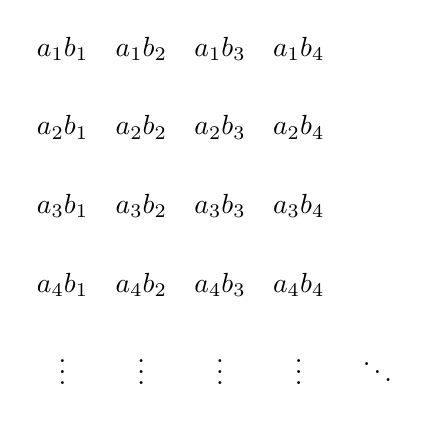
\begin{tikzpicture}
		\term11
		\term12
		\term13
		\term14
		\draw(4,0)node{$\dotso$};
		\term21
		\term22
		\term23
		\term24
		\draw(4,-1)node{$\dotso$};
		\term31
		\term32
		\term33
		\term34
		\draw(4,-2)node{$\dotso$};
		\term41
		\term42
		\term43
		\term44
		\draw(4,-3)node{$\dotso$};
		\draw(0,-4)node{$\vdots$};
		\draw(1,-4)node{$\vdots$};
		\draw(2,-4)node{$\vdots$};
		\draw(3,-4)node{$\vdots$};
		\draw(4,-4)node{$\ddots$};
	\end{tikzpicture}
	\caption{}
	\label{figure:无穷级数.无穷级数乘积各项的矩阵}
\end{figure}

由于级数运算一般不满足交换律和结合律,这就有一个排列的次序与方式的问题.
尽管排列的次序与方式多种多样,
但是最常用的最具应用价值的方式是“对角线”排列与“正方形”排列.

\begin{definition}\label{definition:无穷级数.绝对收敛级数的柯西乘积}
%@see: 《高等数学(第六版 下册)》 P267 定理10
定义级数\(\sum_{n=1}^\infty u_n\)
和\(\sum_{n=1}^\infty v_n\)的\DefineConcept{柯西乘积}为\[
	\left( \sum_{n=1}^\infty u_n \right)
	\cdot
	\left( \sum_{n=1}^\infty v_n \right)
	\defeq
	\sum_{n=1}^\infty \sum_{k=1}^n u_k v_{n-k+1}.
\]
\end{definition}

%@see: 《数学分析(第二版 上册)》(陈纪修) P42
对于正方形排列所得的乘积,
只要\(\sum_{n=1}^\infty u_n\)和\(\sum_{n=1}^\infty v_n\)都收敛,
那么它们的乘积\(\sum_{n=1}^\infty w_n\)总是收敛的.

但是,仅有\(\sum_{n=1}^\infty u_n\)和\(\sum_{n=1}^\infty v_n\)的收敛性,
不足以保证它们的柯西乘积的收敛性.
%@see: 《数学分析(第二版 上册)》(陈纪修) P42 例9.4.7
例如,取\[
	a_n = b_n = \frac{(-1)^{n+1}}{\sqrt{n}}
	\quad(n=1,2,\dotsc),
\]
则级数\(\sum_{n=1}^\infty a_n\)和\(\sum_{n=1}^\infty b_n\)都是条件收敛的,
它们的柯西乘积的一般项为\[
	c_n = (-1)^{n+1} \sum_{i+j=n+1} \frac1{\sqrt{ij}},
\]
注意上面\(c_n\)的表达式中共有\(n\)项,
在每一项中都有\(i+j = n+1\),
因而\[
	\sqrt{ij} \leq \frac{i+j}2 = \frac{n+1}2,
\]
于是得到\[
	\abs{c_n} \geq n \cdot \frac2{n+1},
\]
因此\(\abs{c_n}\)不是无穷小,
级数\(\sum_{n=1}^\infty a_n\)和\(\sum_{n=1}^\infty b_n\)的
柯西乘积\(\sum_{n=1}^\infty c_n\)发散.

\begin{theorem}\label{theorem:无穷级数.绝对收敛级数的柯西乘积必收敛}
%@see: 《数学分析(第二版 上册)》(陈纪修) P42 定理9.4.7
%@see: 《高等数学(第六版 下册)》 P267 定理10
设级数\(\sum_{n=1}^\infty u_n\)和\(\sum_{n=1}^\infty v_n\)都绝对收敛,
其和分别为\(s\)和\(\sigma\),
则它们的柯西乘积也是绝对收敛的,且其和为\(s \cdot \sigma\).
\begin{proof}
设\[
	a_{i_k} b_{j_k}
	\quad(k=1,2,\dotsc)
\]是所有\[
	a_i b_j
	\quad(i=1,2,\dotsc;j=1,2,\dotsc)
\]的任意一种排列,
对任意正整数\(n\),
取\[
	N = \max_{1 \leq k \leq n}\{i_k,j_k\},
\]
则\[
	\sum_{k=1}^n \abs{a_{i_k} b_{j_k}}
	\leq \left(\sum_{i=1}^N \abs{a_i}\right)
	\cdot \left(\sum_{j=1}^N \abs{b_j}\right)
	\leq \left(\sum_{n=1}^\infty \abs{a_n}\right)
	\cdot \left(\sum_{n=1}^\infty \abs{b_n}\right),
\]
因此\(\sum_{k=1}^\infty a_{i_k} b_{j_k}\)绝对收敛.
由\cref{theorem:无穷级数.绝对收敛级数的可交换性} 可知
\(\sum_{k=1}^\infty a_{i_k} b_{j_k}\)的任意更序级数也绝对收敛,且它的和不变.

设\(\sum_{n=1}^\infty d_n\)是
级数\(\sum_{n=1}^\infty a_n\)和\(\sum_{n=1}^\infty b_n\)
按正方形排列所得的乘积,
则\(\sum_{n=1}^\infty d_n\)是
\(\sum_{k=1}^\infty a_{i_k} b_{j_k}\)更序后再添加括号所成的级数,
于是得到\[
	\sum_{k=1}^\infty a_{i_k} b_{j_k}
	= \sum_{n=1}^\infty d_n
	= \left(\sum_{n=1}^\infty a_n\right)
	\cdot \left(\sum_{n=1}^\infty b_n\right)
	= s \cdot \sigma.
	\qedhere
\]
\end{proof}
\end{theorem}

\begin{proposition}\label{theorem:绝对收敛.命题1}
若级数\(\sum_{n=1}^\infty u_n\)绝对收敛,
级数\(\sum_{n=1}^\infty v_n\)条件收敛,
则级数\(\sum_{n=1}^\infty (u_n \pm v_n)\)条件收敛.
\begin{proof}\let\qed\relax
\begin{proof}[证法一]
因为级数\(\sum_{n=1}^\infty u_n\)和\(\sum_{n=1}^\infty v_n\)都收敛,
所以,由\cref{theorem:无穷级数.收敛级数性质2} 可知,
它们相加或相减所得级数\(\sum_{n=1}^\infty (u_n \pm v_n)\)一定收敛.

因为级数\(\sum_{n=1}^\infty v_n\)条件收敛,
所以级数\(\sum_{n=1}^\infty \abs{v_n}\)发散;
由三角不等式 \labelcref{theorem:不等式.三角不等式1} 有\begin{align*}
	\abs{v_n}
	= \abs{(v_n + u_n) - u_n}
	\leq \abs{u_n + v_n} + \abs{u_n}, \\
	\abs{v_n}
	= \abs{(v_n - u_n) + u_n}
	\leq \abs{u_n - v_n} + \abs{u_n};
\end{align*}
于是由\cref{theorem:无穷级数.正项级数的比较审敛法} 可知
级数\(\sum_{n=1}^\infty \left( \abs{u_n \pm v_n} + \abs{u_n} \right)\)发散.

又因为级数\(\sum_{n=1}^\infty u_n\)绝对收敛,
也就是说级数\(\sum_{n=1}^\infty \abs{u_n}\)收敛.
那么由\cref{theorem:无穷级数.收敛级数性质2.推论1} 可知,
级数\[
	\sum_{n=1}^\infty \left[
		\left( \abs{u_n \pm v_n} + \abs{u_n} \right) - \abs{u_n}
	\right]
	= \sum_{n=1}^\infty \abs{u_n \pm v_n}
\]发散.

综上所述,级数\(\sum_{n=1}^\infty (u_n \pm v_n)\)条件收敛.
\end{proof}
\begin{proof}[证法二]
用反证法.
假设级数\(\sum_{n=1}^\infty (u_n \pm v_n)\)绝对收敛,
那么级数\(\sum_{n=1}^\infty \abs{u_n \pm v_n}\)收敛;
加之级数\(\sum_{n=1}^\infty u_n\)绝对收敛,
或者说级数\(\sum_{n=1}^\infty \abs{u_n}\)收敛;
所以由\cref{theorem:无穷级数.收敛级数性质2} 可知,
级数\(\sum_{n=1}^\infty (\abs{u_n + v_n} + \abs{u_n})\)收敛.

又因为\[
	\abs{v_n}
	= \abs{(v_n + u_n) - u_n}
	\leq \abs{u_n + v_n} + \abs{u_n},
\]
所以由\cref{theorem:无穷级数.正项级数的比较审敛法} 可知,
级数\(\sum_{n=1}^\infty \abs{v_n}\)收敛,
也就是说级数\(\sum_{n=1}^\infty v_n\)绝对收敛,矛盾!
因此级数\(\sum_{n=1}^\infty (u_n \pm v_n)\)条件收敛.
\end{proof}
\end{proof}
\end{proposition}

\begin{proposition}\label{theorem:绝对收敛.命题2}
设正项级数\(\sum_{n=1}^\infty u_n\)收敛,
数列\(\{v_n\}\)有界,
则级数\(\sum_{n=1}^\infty u_n v_n\)绝对收敛.
\begin{proof}
设\(\abs{v_n} < M\ (n=1,2,\dotsc)\),
那么\[
	\abs{u_n v_n}
	= \abs{u_n} \abs{v_n}
	< M \abs{u_n}
	= M u_n
	\quad(n=1,2,\dotsc),
\]
于是根据\hyperref[theorem:无穷级数.正项级数的比较审敛法的推论]{正项级数的比较审敛法}可知,
级数\(\sum_{n=1}^\infty u_n v_n\)绝对收敛.
\end{proof}
\end{proposition}

\begin{proposition}\label{theorem:绝对收敛.命题3}
设正项级数\(\sum_{n=1}^\infty u_n\)收敛,
\(\lim_{n\to\infty} v_n = 0\),
则级数\(\sum_{n=1}^\infty u_n v_n\)绝对收敛.
\begin{proof}
根据\cref{theorem:极限.收敛数列的有界性},
数列\(\{v_n\}\)有界.
再根据\cref{theorem:绝对收敛.命题2} 可知
级数\(\sum_{n=1}^\infty u_n v_n\)绝对收敛.
\end{proof}
\end{proposition}

\begin{proposition}\label{theorem:绝对收敛.命题4}
设正项级数\(\sum_{n=1}^\infty u_n\)和\(\sum_{n=1}^\infty v_n\)都收敛,
则级数\(\sum_{n=1}^\infty u_n v_n\)绝对收敛.
\begin{proof}
因为\(\sum_{n=1}^\infty v_n\)收敛,
根据\hyperref[theorem:无穷级数.级数收敛的必要条件]{级数收敛的必要条件},
必有\(\lim_{n\to\infty} v_n = 0\).
于是,根据\cref{theorem:绝对收敛.命题3} 便有
级数\(\sum_{n=1}^\infty u_n v_n\)绝对收敛.
\end{proof}
\end{proposition}

\begin{proposition}\label{theorem:绝对收敛.命题5}
设级数\(\sum_{n=1}^\infty u_n\)绝对收敛,
级数\(\sum_{n=1}^\infty v_n\)条件收敛,
则级数\(\sum_{n=1}^\infty u_n v_n\)绝对收敛.
\begin{proof}
因为级数\(\sum_{n=1}^\infty u_n\)绝对收敛,
所以级数\(\sum_{n=1}^\infty \abs{u_n}\)收敛.
又因为级数\(\sum_{n=1}^\infty v_n\)条件收敛,
所以根据\hyperref[theorem:无穷级数.级数收敛的必要条件]{级数收敛的必要条件}有
\(\lim_{n\to\infty} v_n = 0\).
因此,根据\cref{theorem:绝对收敛.命题3},
级数\(\sum_{n=1}^\infty \abs{u_n} v_n\)绝对收敛,
也就是说,级数\[
	\sum_{n=1}^\infty \abs{\abs{u_n} v_n}
	= \sum_{n=1}^\infty \abs{u_n v_n}
\]收敛,
级数\(\sum_{n=1}^\infty u_n v_n\)绝对收敛.
\end{proof}
\end{proposition}

\begin{example}
设级数\(\sum_{n=1}^\infty u_n^2\)收敛.
证明:级数\(\sum_{n=1}^\infty u_n^3\)绝对收敛.
\begin{proof}
因为级数\(\sum_{n=1}^\infty u_n^2\)收敛,
所以根据\hyperref[theorem:无穷级数.级数收敛的必要条件]{级数收敛的必要条件}有
\(\lim_{n\to\infty} u_n^2 = 0\),
于是\(\lim_{n\to\infty} u_n = 0\).
因此,根据\cref{theorem:绝对收敛.命题3},
级数\(\sum_{n=1}^\infty u_n^2 \cdot u_n
= \sum_{n=1}^\infty u_n^3\)绝对收敛.
\end{proof}
\end{example}
从这个例子出发,我们可以做一些推广.
例如,当级数\(\sum_{n=1}^\infty u_n^3\)收敛时,
级数\(\sum_{n=1}^\infty u_n^4\)未必收敛.
但是,当级数\(\sum_{n=1}^\infty u_n^3\)绝对收敛时,
级数\(\sum_{n=1}^\infty u_n^4\)必定收敛.
还有,当正项级数\(\sum_{n=1}^\infty u_n\)收敛时,
级数\(\sum_{n=1}^\infty \sqrt{u_n}\)未必收敛.

\begin{example}
设级数\(\sum_{n=1}^\infty u_n^2\)收敛,
证明:级数\(\sum_{n=1}^\infty \frac{u_n}{n}\)绝对收敛.
\begin{proof}
因为\[
	\abs{\frac{u_n}{n}}
	= \abs{u_n} \cdot \frac{1}{n}
	\leq \frac12 \left( u_n^2 + \frac{1}{n^2} \right),
\]
加之级数\(\sum_{n=1}^\infty \frac{1}{n^2}\)收敛,
所以级数\(\sum_{n=1}^\infty \abs{\frac{u_n}{n}}\)收敛.
\end{proof}
\end{example}
